%! TEX root = ex_plot.tex

%% LaTeX tips and stuff.
%% Made for you not to spend long hours on Google and StackOverflow to look weird stuff up.
%%
%% Copyright 2020 Riccardo Milani
%%
%% Licensed under the "THE BEER-WARE LICENSE" (Revision 42):
%% Riccardo Milani wrote this file. As long as you retain this notice you
%% can do whatever you want with this stuff. If we meet some day, and you think
%% this stuff is worth it, you can buy me a beer or coffee in return


% Authors: Riccardo Milani, X12

% Acknowledgments: Cl\'ement Colas, Ga\"etan Mangeon, Germain Davy

\documentclass[a4paper,11pt]{article}

\usepackage[centering,scale=0.9]{geometry}

\usepackage[svgnames,table]{xcolor} % Possibly useless here

\usepackage{tikz} % useless, since pgfplots already loads it
\usetikzlibrary{calc} % It allows to make arithmetic operations with TiKz nodes.
\usetikzlibrary{spy} % Spy / zoom / magnifying tools
\usetikzlibrary{decorations.footprints} % Decorations
\usepackage{pgfplots} % useless, since pgfplotstable already loads it
\usepgfplotslibrary{patchplots} % 3D plots with patches different than squares
\usepackage{pgfplotstable}
\usepgflibrary{plotmarks} % Extended use of plot markers
\usepgfplotslibrary{groupplots}
\pgfplotsset{compat=newest,
width=11cm,
% Plot canvas style
graph/.style={grid=major, major grid style=dotted},
% Plot style
%forcsv/.style={col sep=comma}, % If comma-separated values
ana/.style={thin,color=black,mark=none},
gridone/.style={thick,color=blue,mark=square},
gridtwo/.style={thick,color=red,mark=diamond},
gridthree/.style={thick,color=green,mark=triangle},
every n index/.style={
  each nth point=#1,% This should be enough: the following two lines discard the warnings
  filter discard warning=false,
  unbounded coords=jump
},
colormap={mypalette}{color={Navy} color={Olive} color={DarkMagenta}},
} % pgfplotsset

% For the fancy colorful table
\usepackage{booktabs}
\xdefinecolor{blue-rule}{RGB}{0,26,112}
\xdefinecolor{blue-table-bg}{RGB}{194 214 241}
%% Odd columns
\newcolumntype{O}{>{\columncolor{white}}c}%
%% Even columns
\newcolumntype{E}{>{\columncolor{blue-table-bg}}c}%
%% Horizontal spacing
\setlength{\tabcolsep}{25pt}
% New environment for rounded tables
\usepackage{environ}
\NewEnviron{roundtable}[1]{%
    \noindent%
    \begin{tikzpicture}[line width=.1mm,rounded corners=.5em]
      \node[clip,inner sep=.5\pgflinewidth] (table) {%
        \begin{tabular}{#1}
          \BODY%
        \end{tabular}%
      };
    \end{tikzpicture}%
  }

% Method one: read and store
\pgfplotstableread{grid1.dat}\gridone

\begin{document}
  \begin{center}
    \begin{tikzpicture}
      \begin{scope}[spy using outlines,connect spies]
        \begin{axis}[name=graph_one,%
          graph,title={Title $\alpha$},xlabel={\large Time [s]},ylabel={\small Interface position [mm]},legend,legend pos=south east,legend style={fill=none,draw=red}%
          ]
          \addplot[ana] table[x index=0,y index=1] {analytical.dat};

          % Method one: read and store - follows
          %\addplot[gridone,every n index=20] table[x index=0,y index=1] {\gridone};
          % ...If columns have names
          %\addplot[gridone,every n index=20] table[x=xname,y=yname] {\gridone};
          % ...Filter marks, not data point
          \addplot[gridone,mark repeat=20] table[x index=0,y index=1] {\gridone};\label{grp:gr1}
          % Method two: read, plot, discard
          \addplot[gridtwo,every n index=20] table[x index=0,y index=1] {grid2.dat};
          % Method three: read a file with only two columns the first is x the second y
          % % Faster than method two, but does not allow data manipulation
          \addplot[gridthree,every n index=20] file {grid3.dat};
          % Legend
          \legend{analytical,Grid 1,Grid 2,Grid 3}
          % Operation with data
          \addplot[gridone,every n index=20,dashed,mark options={solid}] table[x index=0,y expr={\thisrowno{1}/3}] {\gridone};
          \addlegendentry{Grid 1 bis}
          \addplot[gridtwo,every n index=20,dotted,mark options={solid}] table[x index=0,y expr={\thisrowno{1}/3+1e-4}] {grid2.dat};
          \addplot[gridthree,every n index=20,dashdotted,mark options={solid}] table[x index=0,y expr={\thisrowno{1}/3+2e-4}] {grid3.dat};
          \coordinate (tospy)    at (4,2.1e-4);
          \coordinate (location) at (10,8e-4);
        \end{axis}
        \spy [magnification=3,size=2cm,circle] on (tospy) in node at (location);
      \end{scope}
    \end{tikzpicture}
  \end{center}

  You can even do this: \ref{grp:gr1} Grid 1.\par
  \begin{center}
    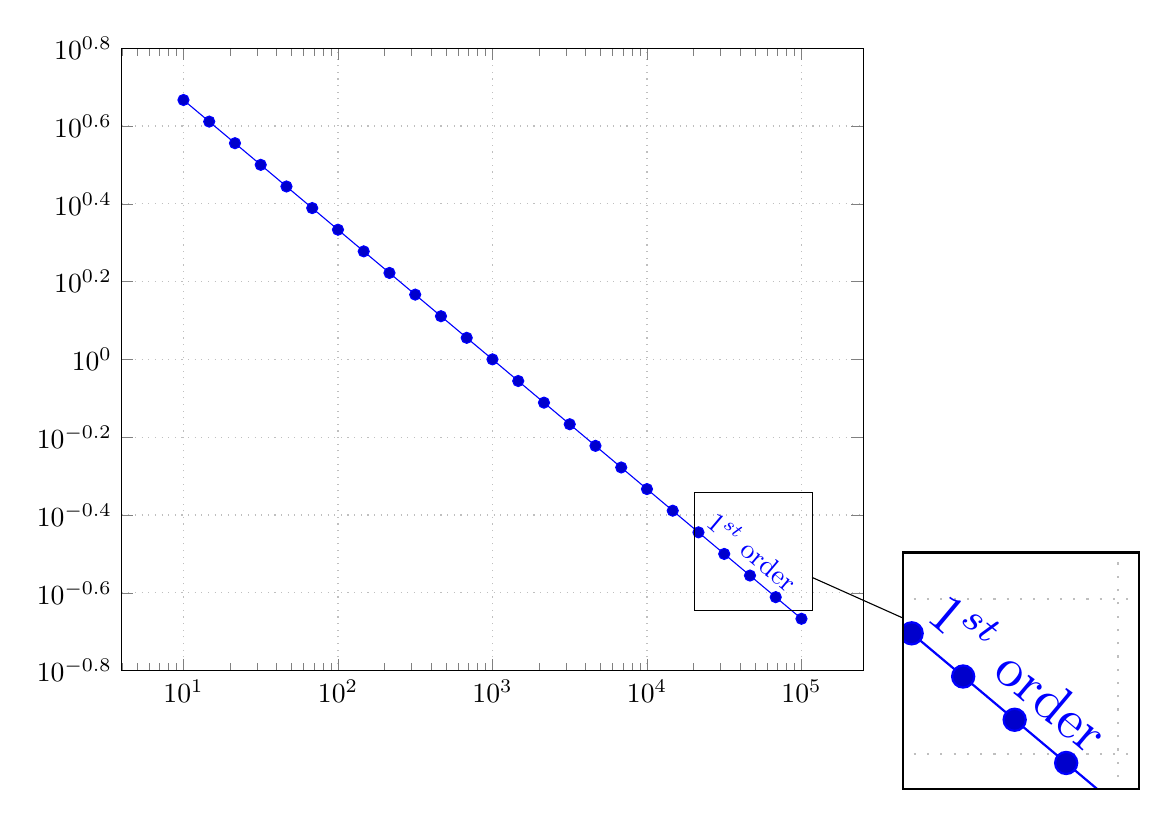
\begin{tikzpicture}
      \begin{scope}[spy using outlines,connect spies]
        \begin{loglogaxis}[name=gt,graph]
          \addplot expression[domain=1e1:1e5] {10*x^(-1/3)} node[above,sloped,pos=0.9] (inside) {$1^{st}$ order};
        \end{loglogaxis}
        \coordinate (outside) at ($(gt.south east)+(2,0)$);
        \spy[magnification=2,size=3cm,rectangle] on (inside) in node at (outside);
      \end{scope}
    \end{tikzpicture}
  \end{center}
  \clearpage

  Grouping up plots:\par
  \begin{center}
    \begin{tikzpicture}
      \begin{groupplot}[%
        group style={%
          group size=2 by 2,
          xlabels at=edge bottom,
          ylabels at=edge left
        },
        % The following applies to every subplot
        width=0.48\linewidth,graph,
        ymin=1e-5,ymax=1e-3,
        xlabel={\large Time [s]},ylabel={\small Interface position [mm]},
        ]
        \nextgroupplot
          \addplot[gridone,mark repeat=20] table[x index=0,y index=1] {grid1.dat};
        \nextgroupplot
          \addplot[gridtwo,every n index=20] table[x index=0,y index=1] {grid2.dat};
        \nextgroupplot
          \addplot[gridthree,every n index=20] table[x index=0,y index=1] {grid3.dat};
        \nextgroupplot[group/empty plot] % Leave an empty plot
      \end{groupplot}
    \end{tikzpicture}
  \end{center}

  You may wonder: the 2D version is too easy. Here you are\par
  \begin{center}
    \begin{tikzpicture}
      \begin{axis}[%
        %title style={align=center},
        tick pos = left,%
        xmin=1, xmax=5,%
        xtick={1,2,3,4,5},%
        %scaled x ticks=base 10:-3,%
        ymin=100, ymax=700,%
        ytick={100,300,500,700},%
        %scaled y ticks=base 10:-3,%
        zmin=0, zmax=1.5e-3,%
        ztick={0,0.5e-3,1e-3,1.5e-3},%
        %scaled z ticks=base 10:-3,%
        enlarge x limits=0.1,%
        enlarge y limits=0.1,%
        enlarge z limits=0.1,%
        y dir=reverse,% Reverse direction, higher values at the front
        legend,legend pos=north east,legend cell align={left},legend style={font=\color{gray}\small},%
        view={20}{25}, % Change the 3D view of the plot
        ]
        \addplot3 [surf,shader=flat,draw=black,fill=black,draw opacity=0.5,fill opacity=0.5] coordinates {(1,100,5.8e-4) (1,700,5.8e-4)

                                                                                                          (5,100,5.8e-4) (5,700,5.8e-4)};
        \addplot3 [surf,shader=faceted,colormap/bluered,draw opacity=0.5,fill opacity=0.5] table {results.dat};
        \addplot3 [black,opacity=0.5] coordinates {(1.00, 312.3, 5.80e-4)
                                                   (1.07, 300.0, 5.80e-4)
                                                   (1.74, 200.0, 5.80e-4)
                                                   (2.00, 174.6, 5.80e-4)
                                                   (3.00, 117.1, 5.80e-4)
                                                   (3.37, 100.0, 5.80e-4)};
        %mark=square,mark options={draw=black,fill=white}
        \legend{A plane,My surface,Intersection}
      \end{axis}
    \end{tikzpicture}
  \end{center}
  \clearpage

  You see, by default, a square patch is assumed, but look at these triangles (you are right, colors are not great, but, hey, I set them randomly)\par
  \begin{center}
    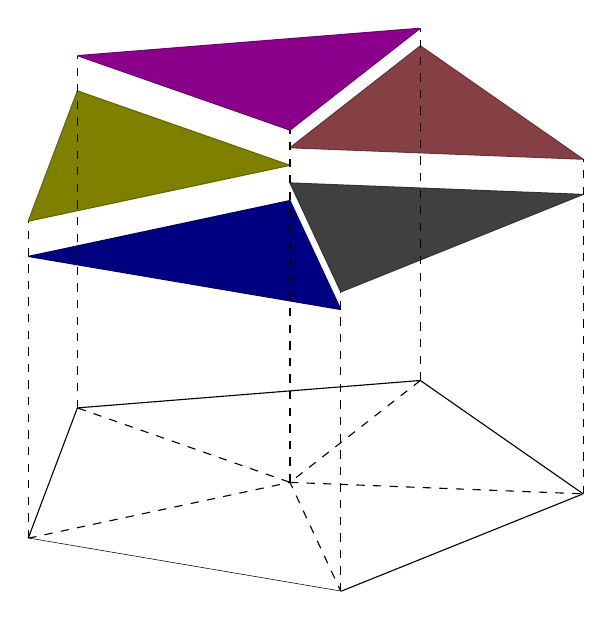
\begin{tikzpicture}
      \begin{axis}[zmin=0,zmax=2,axis x line=none,axis y line=none,axis z line=none]
        \addplot3 [surf,
          patch,patch type=triangle, % activate patch and set type
          colormap name=mypalette, % choose the colormap
          point meta min=1.6,point meta max=2, % set the extrema of the colormap
          ]
          coordinates {
            (0,1,2.0)                  (0,0,2.0) (-0.951056,+0.309016,2.0)

            (0,1,1.9)                  (0,0,1.9) (+0.951056,+0.309016,1.9)

            (-0.951056,+0.309016,1.8)  (0,0,1.8) (-0.587785,-0.809016,1.8)

            (+0.951056,+0.309016,1.7)  (0,0,1.7) (+0.587785,-0.809016,1.7)

            (-0.587785,-0.809016,1.6)  (0,0,1.6) (+0.587785,-0.809016,1.6)
          };
        \addplot3[black,mark=none] coordinates { (0,1,0) (-0.951056,+0.309016,0) (-0.587785,-0.809016,0)
          (+0.587785,-0.809016,0) (+0.587785,-0.809016,0) (+0.951056,+0.309016,0) (0,1,0)};
        \addplot3[thin,dashed,black] coordinates {(0,1,0)                 (0,0,0) (-0.951056,+0.309016,0)};
        \addplot3[thin,dashed,black] coordinates {(-0.587785,-0.809016,0) (0,0,0) (+0.587785,-0.809016,0)};
        \addplot3[thin,dashed,black] coordinates {(0,0,0) (+0.951056,+0.309016,0)};
        \addplot3[thin,dashed,black] coordinates {(0,0,0) (0,0,2)};
        \addplot3[thin,dashed,black] coordinates {(0,1,0) (0,1,2)};
        \addplot3[thin,dashed,black] coordinates {(-0.951056,+0.309016,0) (-0.951056,+0.309016,2)};
        \addplot3[thin,dashed,black] coordinates {(+0.951056,+0.309016,0) (+0.951056,+0.309016,1.9)};
        \addplot3[thin,dashed,black] coordinates {(-0.587785,-0.809016,0) (-0.587785,-0.809016,1.8)};
        \addplot3[thin,dashed,black] coordinates {(+0.587785,-0.809016,0) (+0.587785,-0.809016,1.7)};
      \end{axis}
    \end{tikzpicture}
  \end{center}

  And now, a table with \texttt{pgfplotstable}.\par
  % The following definitions may be put inside the square brackets in the pgfplotstabletypeset, but here are globally defined, hence re-usable
  \pgfplotstableset{%
    datastyle/.style={sci,sci zerofill=true,precision=3,},
    columns/mesh/.style={column name={},string type,column type={c|}},
    columns/cenhho/.style={column name={$a_{h}^{c}$},datastyle,column type={c}},
    columns/cencdo/.style={column name={$a_{c}^{c}$},datastyle,column type={c|}},
    columns/upwhho/.style={column name={$a_{h}^{u}$},datastyle,column type={c}},
    columns/upwcdo/.style={column name={$a_{c}^{u}$},datastyle,column type={c}},
  }
  \begin{center}
  \pgfplotstabletypeset[%
    columns={mesh,cenhho,cencdo,upwhho,upwcdo},
    every head row/.append style={after row=\hline,before row={ Mesh & \multicolumn{2}{c|}{Centered} & \multicolumn{2}{c}{Upwind}\\}},
    ]
  {mesh  cenhho       cencdo      upwhho      upwcdo
   H4    3.18574e-01  3.18574e-01 3.20767e-01 3.19698e-01
   H8    1.04893e-01  1.04893e-01 1.07353e-01 1.06905e-01
   H16   2.81905e-02  2.81905e-02 2.99132e-02 2.97545e-02
   H32   7.17828e-03  7.17828e-03 8.24024e-03 8.18674e-03
   H64   1.80288e-03  1.80056e-03 2.45854e-03 2.43920e-03
  }
  \end{center}

  Creating columns, computing orders of convergence, sorting, some styles,\ldots all in the following example.
  \pgfplotstablesort[sort key={dofs}]{\testing}{%
    err         dofs
    2.5e-1      4
    1           1
    1.5645e-2   64
    6.15e-2     16
  }
  \pgfplotstablecreatecol[create col/dyadic refinement rate={dofs}]{refdofs}{\testing}
  \pgfplotstablecreatecol[create col/dyadic refinement rate={err}]{referr}{\testing}
  \begin{center}
    \pgfplotstabletypeset[%
      columns={err,dofs,ord},
      every head row/.style={after row={\hline}},
      %sort,sort key={dofs},
      columns/err/.style={column name={Errors},sci,sci zerofill=true,precision=6,dec sep align},
      columns/dofs/.style={column name={\#DoFs},column type={c|},int detect},
      % Separate creation and style definition
      create on use/ord/.style={create col/expr={-2*\thisrow{referr}/\thisrow{refdofs}}},
      columns/ord/.style={column name={Order cvg (2D)},precision=2,fixed zerofill},
      ]{\testing}
  \end{center}
  \clearpage

  What about some textual plot?\\
  \noindent Here you are!
  \newcommand{\axisfontsize}{\normalsize}
  \newcommand{\tickfontsize}{\footnotesize}

  \def\xShift{-2.5cm}
  \def\yShift{-1.7cm}

  \begin{center}
    \begin{tikzpicture}
      \begin{axis}
        [
        name=mg,
        % Dimension and scaling
        xmin=0,xmax=1.1,ymin=0,ymax=1.1,
        unit vector ratio=3 2,
        % Axis and labels
        axis lines*=center,
        % % x
        xlabel={$u$-$p$ coupling},
        xlabel style={font=\axisfontsize,at={(ticklabel cs:1)},anchor=east,yshift=-4pt},
        % % x
        ylabel={Nonlinearity},
        ylabel style={font=\axisfontsize,at={(ticklabel cs:1)},anchor=east},
        % Ticks
        % % x
        xtick={0.15,0.7,1},
        xticklabels={AC\\1 step,AC\\$n$ step,Monolithic},
        xticklabel style={font=\tickfontsize,align=center},
        % % x
        ytick={0.10,0.3,0.8,1},
        yticklabel style={font=\tickfontsize,align=right},
        yticklabels={Explicit\\advection,Picard\\1 step,Picard\\(converged),Newton},
        %
        after end axis/.code={
           \draw (rel axis cs:0,0.4) +(-2mm,-1mm) -- +(2mm,1mm)
                ++(0pt,-1mm)
                +(-2mm,-1mm) -- +(2mm,1mm)
                (rel axis cs:0.4,0) +(-1mm,-2mm) -- +(1mm,2mm)
                ++(-1mm,0pt)
                +(-1mm,-2mm) -- +(1mm,2mm)
                ;
           }
        ]
        \newcommand{\ptAC}{(0.15,0.1)}
        \newcommand{\ptFC}{(1,0.8)}
        \newcommand{\ptIn}{(1,0.1)}
        \pgfplotsinvokeforeach{xcomb,ycomb}{
          \addplot[densely dotted,very thick,opacity=0.2,#1] coordinates {\ptAC};
          \addplot[densely dotted,very thick,opacity=0.2,#1] coordinates {\ptFC};
          \addplot[densely dotted,very thick,opacity=0.2,#1] coordinates {\ptIn};
        }
        \draw[black,fill=white] \ptAC circle (0.1cm);
        \node[pin=above:{AC-based}] at \ptAC {};
        %\addplot[densely dotted,very thick,opacity=0.2,xcomb] coordinates {(0.15,0.1)};
        %\node [fill=blue,above,font=\tickfontsize] at (0.15,0.1) {AC-based};
        \draw[fill=black] \ptFC circle (0.1cm);
        \node[pin=above left:{Fully coupled}] at \ptFC {};
        %\node [fill=black,] at (1,1) {};
        \draw[fill=gray] \ptIn circle (0.1cm);
        \node[pin=above left:{Intermediate}] at \ptIn {};

      \end{axis}
      \draw[<-|] ([xshift=\xShift]mg.north west) node [rotate=90,below,font=\tickfontsize] {expensive}
                --                              node [midway,rotate=90,below,font=\axisfontsize] {cost}
                ([xshift=\xShift]mg.south west) node [rotate=90,below,font=\tickfontsize] {cheap};
      \draw[<-|] ([yshift=\yShift]mg.south east) node [above,font=\tickfontsize] {expensive}
                --                              node [midway,above,font=\axisfontsize] {cost}
                ([yshift=\yShift]mg.south west) node [above,font=\tickfontsize] {cheap};
      \node [below,font=\tickfontsize] at ([yshift=\yShift]mg.south west) {approximated};
      \node [below,font=\axisfontsize] at ([yshift=\yShift]mg.south) {incompressibility constraint};
      \node [below,font=\tickfontsize] at ([yshift=\yShift]mg.south east) {accurate};
    \end{tikzpicture}
  \end{center}

  And now a fancy colorful table (in order to have a float, put it inside a \texttt{table} environment)\\
\setlength\arrayrulewidth{2.2pt}%
\arrayrulecolor{blue-rule}
%% Vertical spacing
\renewcommand{\arraystretch}{1.2}
  \begin{roundtable}{O|E|O|E}
   \rowcolor{blue-rule}%
      {\color{white}Puissance nominale} & {\color{white}Surface rotor} & {\color{white}Type} & {\color{white}Production annuelle}\\
    \hline
    1 kW & 7 m$^2$ & vertical & 1000 kWh \\
    \hline
    1 kW & 7 m$^2$ & vertical & 1000 kWh \\
    \hline
    1 kW & 7 m$^2$ & vertical & 1000 kWh \\
    \hline
    1 kW & 7 m$^2$ & vertical & 1000 kWh
  \end{roundtable}

  Let's play a game: treasure hunting (or \texttt{tikz} decorations)
  \begin{center}
    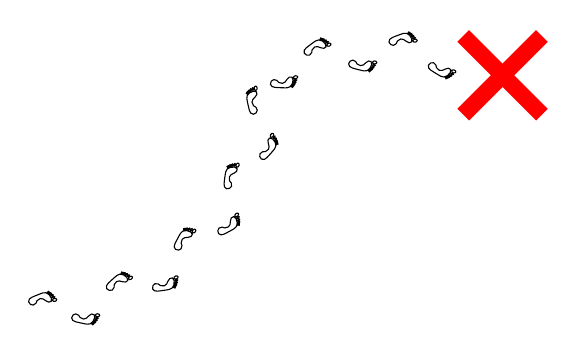
\begin{tikzpicture}[decoration={footprints}]
      \draw[decorate] (0,0) to[bend right=45] (3,3) to[bend left=20] (6,3);
      \draw[color=red, line width=6pt] (5.5,3.5) -- (6.5,2.5);
      \draw[color=red, line width=6pt] (5.5,2.5) -- (6.5,3.5);
    \end{tikzpicture}
  \end{center}

  \clearpage
  Another game: archery - an example of looping and conditionals

  \begin{center}
    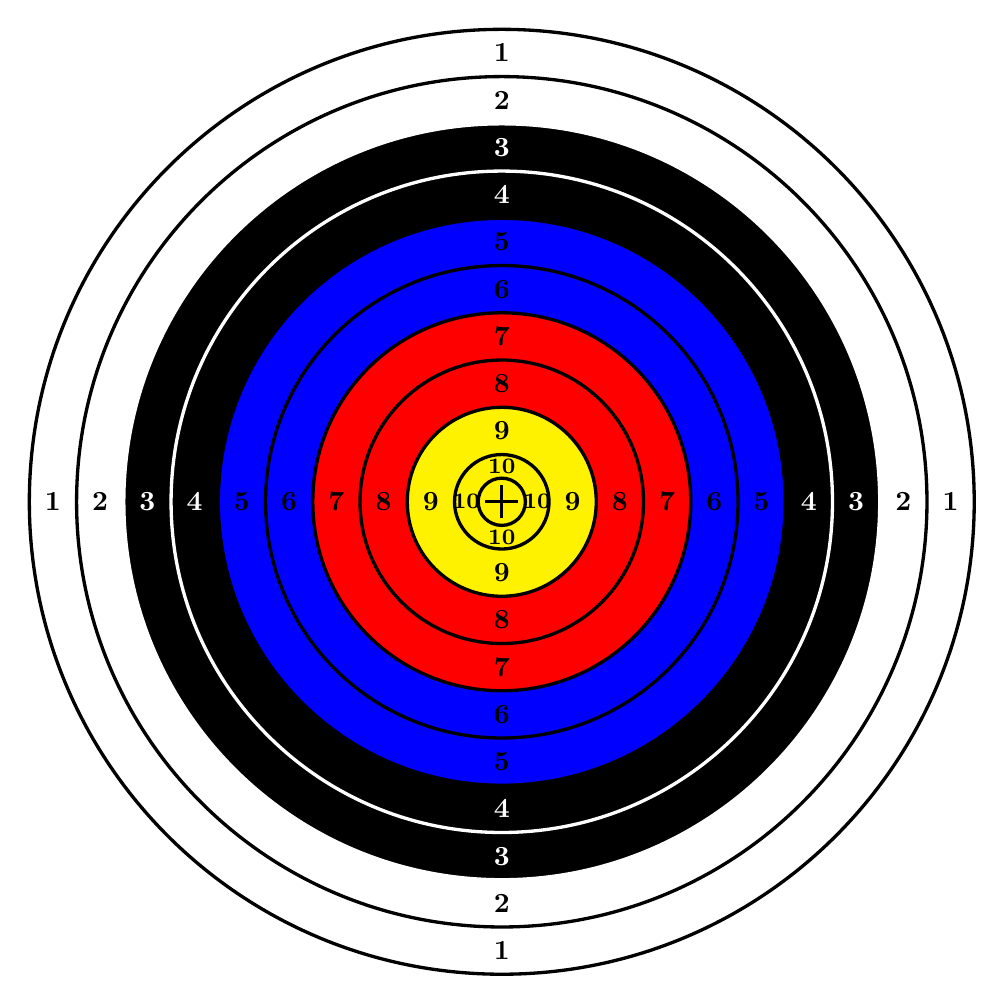
\begin{tikzpicture}[
        scale=0.3,
        tgtline/.style={line width=1.2pt},
        target/.style 2 args={tgtline,
                             fill=#1,draw=#2},
        target/.default={white}{black},
        tgtnumbers/.style 2 args={color=#1,font={#2},},
        tgtnumbers/.default={black}{\bfseries},
      ]
      \foreach \l\fl\cl in {0/white/black,1/black/white,2/blue/black,3/red/black,4/yellow/black}{
        \foreach \j in {0,1} {
          % Inwards so that smaller circles cover the bigger ones (instead of being covered by them)
          \pgfmathsetmacro\crcl{20-4*\l-2*\j}
          \draw[target={\fl}{\cl}] (0,0) circle (\crcl);
          \pgfmathsetmacro\posnum{\crcl-1}
          \pgfmathtruncatemacro\printnum{2*\l+\j+1}
          % 10 is a special case
          \ifnum \numexpr \printnum < 10
            \foreach \jj in {\posnum,-\posnum}{
              \node[tgtnumbers={\cl}{\bfseries}] at (0,\jj) {\printnum};
              \node[tgtnumbers={\cl}{\bfseries}] at (\jj,0) {\printnum};
            }
          \fi
        }
      }
      % 10s
      \newcommand{\tencl}{black}
      \draw[target={none}{\tencl}] (0,0) circle (1);
      \foreach \jj in {1.5,-1.5}{
        \node[tgtnumbers={\tencl}{\footnotesize\bfseries}] at (0,\jj) {10};
        \node[tgtnumbers={\tencl}{\footnotesize\bfseries}] at (\jj,0) {10};
      }
      % Inner Cross
      \draw[tgtline,draw=black] (0.7,0) -- (-0.7,0);
      \draw[tgtline,draw=black] (0,0.7) -- (0,-0.7);
    \end{tikzpicture}
  \end{center}

\end{document}
